\documentclass[10pt,a4paper,oneside,russian]{article}
\usepackage[utf8x]{inputenc}
\usepackage{cmap}
\usepackage{textgreek}
\usepackage[russian]{babel}
\usepackage[T2A]{fontenc}
\usepackage{amsmath}
\usepackage{amsfonts}
\usepackage{amssymb}
\usepackage{listingsutf8}
\usepackage[usenames,dvipsnames,svgnames,table]{xcolor}
\usepackage[left=1.5cm,right=1.5cm,top=1.5cm,bottom=2.5cm,bindingoffset=0cm]{geometry}
\usepackage{fancyhdr}
\usepackage{graphicx}
\usepackage{listings}
\lstloadlanguages{[5.2]Mathematica}
\lstset{basicstyle=\small}

\lstdefinestyle{customc}{
  belowcaptionskip=1\baselineskip,
  breaklines=true,
  frame=L,
  xleftmargin=\parindent,
  language=Mathematica,
  showstringspaces=false,
  basicstyle=\footnotesize\ttfamily,
  keywordstyle=\bfseries\color{green},
  commentstyle=\itshape\color{black},
  identifierstyle=\color{blue},
  stringstyle=\color{orange},
}
\lstset{escapechar=@,style=customc,escapeinside={\%*}{*)},}

\makeatletter

\newcommand{\abs}[1]{
  \left\vert #1 \right\vert
}

\begin{document}
\begin{titlepage}
  \begin{center}
    % Upper part of the page
    \textbf{\large МИНИСТЕРСТВО ОБРАЗОВАНИЯ РЕСПУбЛИКИ БЕЛАРУСЬ} \\[1.0cm]
    \textbf{\large БЕЛОРУССКИЙ ГОСУДАРСТВЕННЫЙ УНИВЕРСИТЕТ} \\[1.0cm]
    \textbf{\large Факультет прикладной математики и информатики} \\[4.7cm]
    %    \textbf{\large Кафедра вычислетельной математики}\\[4.5cm]

    % Title
    \Large Павлович Владислав Викторович \\[0.2cm]
    \textbf{\LARGE МЕТОДЫ ЧИСЛЕННОГО АНАЛИЗА}\\[1.0cm]
    \textbf{\Large Отчёт по лабораторной работе №1\\
      студента 3 курса 3 группы} \\[3.5cm]

    %supervisor
    \begin{flushright} \large
      \emph{Преподаватель:} \\
      \textsc{Полещук Максим Александрович}
    \end{flushright}
    \vfill

    % Bottom of the page
    \textbf{\large {Минск, 2016}}
  \end{center}
  \thispagestyle{empty}
\end{titlepage}
\begin{titlepage}
  \tableofcontents
  \thispagestyle{empty}
\end{titlepage}

\section{Задание 1}
Классическим методом Рунге-Кутты четвёртого порядка точности найти приближенное
решение задачи Коши дифференциального уравнения:
\begin{align*}
  &u' = -(g + 0.05s)x^{g-1+0.05s}u\sin(x^{g+0.05s}), u(0) = e, g = 3, s = 2,\\
  &u' = -3.1x^{2.1}u\sin(x^{3.1})
\end{align*}

\section{Теория}
Была использована следующая совокупность формул для метода Рунге-Кутты четвёртого
порядка точности:
\begin{align*}
  &k_1 = hf(x, y),\\
  &k_2 = hf\left(x + \dfrac{h}{2}, y + \dfrac{k_1}{2}\right),\\
  &k_3 = hf\left(x + \dfrac{h}{2}, y + \dfrac{k_2}{2}\right),\\
  &k_4 = hf(x + h, y + k_3),\\
  &y(x + h) = y(x) + \dfrac{1}{6}(k_1 + 2k_2 + 2k_3 + k_4),\\
\end{align*}

Новое $h$ вычисляется по следующей формуле:
\begin{align*}
  h_{\varepsilon} = \dfrac{h}{2}\sqrt{\dfrac{(2^k - 1)\varepsilon}{\left|y_{h/2} - y_h\right|}}
\end{align*}

\section{Результаты}
Число итераций: $N = 2601$, максимальная ошибка: $E_{gl} = 3.83854e-05$.\\
  \begin{tabular}{|c|c|c|c|}
    \hline
    i &h &|u(x)-y(xn)| &$\left|\dfrac{u(x) - y(xn)}{u(x)}\right|$\\\hline
1&0.0005&0&0\\ \hline
2&0.0005&0&0\\ \hline
3&0.0005&0&0\\ \hline
4&0.0005&0&0\\ \hline
5&0.0005&0&0\\ \hline
6&0.0005&0&0\\ \hline
7&0.0005&0&0\\ \hline
8&0.0005&0&0\\ \hline
9&0.0005&0&0\\ \hline
10&0.0005&0&0\\ \hline
11&0.0005&0&0\\ \hline
12&0.0005&0&0\\ \hline
13&0.0005&0&0\\ \hline
14&0.0005&0&0\\ \hline
15&0.0005&0&0\\ \hline
16&0.0005&0&0\\ \hline
17&0.0005&0&0\\ \hline
18&0.0005&0&0\\ \hline
19&0.0005&0&0\\ \hline
20&0.0005&0&0\\ \hline
N-19&0.000499964&3.31998e-05&6.01572e-05\\ \hline
N-18&0.000499964&3.32594e-05&6.03937e-05\\ \hline
N-17&0.000499964&3.31998e-05&6.04139e-05\\ \hline
N-16&0.000499964&3.32594e-05&6.06511e-05\\ \hline
N-15&0.000499964&3.31998e-05&6.0671e-05\\ \hline
N-14&0.000499964&3.32594e-05&6.09089e-05\\ \hline
N-13&0.000499964&3.32594e-05&6.1038e-05\\ \hline
N-12&0.000499964&3.31998e-05&6.10576e-05\\ \hline
N-11&0.000499964&3.31998e-05&6.11867e-05\\ \hline
N-10&0.000499964&3.3319e-05&6.1536e-05\\ \hline
N-9&0.000499964&3.3319e-05&6.16658e-05\\ \hline
N-8&0.000499964&3.3319e-05&6.17957e-05\\ \hline
N-7&0.000499964&3.3319e-05&6.19257e-05\\ \hline
N-6&0.000499964&3.33786e-05&6.21668e-05\\ \hline
N-5&0.000499964&3.32594e-05&6.20747e-05\\ \hline
N-4&0.000499964&3.3319e-05&6.23163e-05\\ \hline
N-3&0.000499964&3.33786e-05&6.25583e-05\\ \hline
N-2&0.000499964&3.3319e-05&6.25771e-05\\ \hline
N-1&0.000499964&3.33786e-05&6.28199e-05\\ \hline
N-0&2.98023e-06&3.3319e-05&6.27085e-05\\ \hline
  \end{tabular}

  \begin{tabular}{|c|c|c|c|}
    \hline
    $i$ & $u_i$ & $f(x_i)$ & $\Delta_i$\\ \hline
    1&2.71828&2.71828&0\\ \hline
2&2.71828&2.71828&0\\ \hline
3&2.71828&2.71828&0\\ \hline
4&2.71828&2.71828&0\\ \hline
5&2.71828&2.71828&0\\ \hline
6&2.71828&2.71828&0\\ \hline
7&2.71828&2.71828&0\\ \hline
8&2.71828&2.71828&0\\ \hline
9&2.71828&2.71828&0\\ \hline
10&2.71828&2.71828&0\\ \hline
11&2.71828&2.71828&0\\ \hline
12&2.71828&2.71828&0\\ \hline
13&2.71828&2.71828&0\\ \hline
14&2.71828&2.71828&0\\ \hline
15&2.71828&2.71828&0\\ \hline
16&2.71828&2.71828&0\\ \hline
17&2.71828&2.71828&0\\ \hline
18&2.71828&2.71828&0\\ \hline
19&2.71828&2.71828&0\\ \hline
20&2.71828&2.71828&0\\ \hline
N-19&0.55185&0.55185&0\\ \hline
N-18&0.550676&0.550676&0\\ \hline
N-17&0.549506&0.549506&0\\ \hline
N-16&0.54834&0.54834&0\\ \hline
N-15&0.547177&0.547177&0\\ \hline
N-14&0.546018&0.546018&0\\ \hline
N-13&0.544863&0.544863&0\\ \hline
N-12&0.543712&0.543712&3.97364e-09\\ \hline
N-11&0.542565&0.542565&3.97364e-09\\ \hline
N-10&0.541422&0.541422&0\\ \hline
N-9&0.540282&0.540282&0\\ \hline
N-8&0.539147&0.539147&0\\ \hline
N-7&0.538015&0.538015&0\\ \hline
N-6&0.536887&0.536887&0\\ \hline
N-5&0.535763&0.535763&3.97364e-09\\ \hline
N-4&0.534643&0.534643&0\\ \hline
N-3&0.533526&0.533526&0\\ \hline
N-2&0.532414&0.532414&0\\ \hline
N-1&0.531305&0.531305&0\\ \hline
N-0&0.531298&0.531298&3.97364e-09\\ \hline

  \end{tabular}

\section{Задание 2}
Экстраполяционным методом Адамса четвёртого порядка точности найти приближённое
решение задачи Коши дифференциального уравнения из задания 1 на сетке узлов с
фиксированным шагом $h = 5 \cdot 10^{-3}$ построив начало таблицы с использованием метода Рунге-Кутты.
\section{Теория}
Была использована следующая формула для экстраполяционного метода Адамса с $q = 3$:
\begin{align*}
  y_{n + 1} = y_n + \dfrac{h}{24}(55f_n - 59f_{n - 1} + 37f_{n - 2} - 9f_{n - 3}).
\end{align*}

\section{Результаты}
\begin{enumerate}
  \item Максимальная глобальная ошибка: $3.82662e-05$.
  \item $251 / (720 * 5^5) * max|u^{(5)}| = 0.0081791$.
  \item Приближённые значения $y_n$:\\
  \begin{tabular}{|c|c|}
    \hline
    $i$ & $y_i$\\ \hline
    1&2.71828\\ \hline
    2&2.71828\\ \hline
    3&2.71828\\ \hline
    4&2.71828\\ \hline
    5&2.71828\\ \hline
    6&2.71828\\ \hline
    7&2.71828\\ \hline
    8&2.71828\\ \hline
    9&2.71828\\ \hline
    10&2.71828\\ \hline
    11&2.71828\\ \hline
    12&2.71828\\ \hline
    13&2.71828\\ \hline
    14&2.71828\\ \hline
    15&2.71828\\ \hline
    16&2.71828\\ \hline
    17&2.71828\\ \hline
    18&2.71828\\ \hline
    19&2.71828\\ \hline
    20&2.71828\\ \hline
    N-19&0.55185\\ \hline
    N-18&0.550676\\ \hline
    N-17&0.549506\\ \hline
    N-16&0.548339\\ \hline
    N-15&0.547177\\ \hline
    N-14&0.546018\\ \hline
    N-13&0.544863\\ \hline
    N-12&0.543712\\ \hline
    N-11&0.542565\\ \hline
    N-10&0.541422\\ \hline
    N-9&0.540282\\ \hline
    N-8&0.539146\\ \hline
    N-7&0.538015\\ \hline
    N-6&0.536887\\ \hline
    N-5&0.535763\\ \hline
    N-4&0.534642\\ \hline
    N-3&0.533526\\ \hline
    N-2&0.532413\\ \hline
    N-1&0.531305\\ \hline
    N-0&0.5302\\ \hline
  \end{tabular}

  \begin{center}
    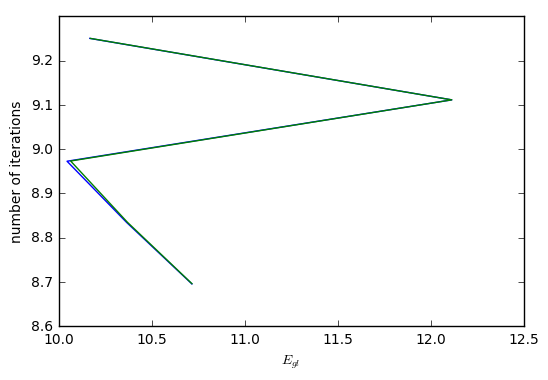
\includegraphics[scale=0.60]{errors-plot.png}
  \end{center}
\end{enumerate}

\section{Исходный код}
\lstinputlisting{runge_kutta.cpp}
\end{document}
